% Local numeric construction example, not source data. Replace every object.
% Compute derived coordinates first; preserve the actual original relations.
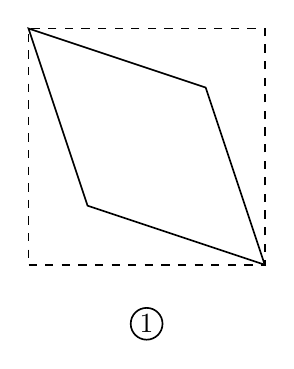
\begin{tikzpicture}[x=1cm,y=1cm,font=\normalsize,
 geometry edge/.style={solid,line width=.6pt},
 geometry mark/.style={solid,line width=.6pt},
 geometry label/.style={font=\normalsize,inner sep=2pt}]
\coordinate (Q1) at (0,0);
\coordinate (Q2) at (3,0);
\coordinate (Q3) at (3,3);
\coordinate (Q4) at (0,3);
\coordinate (P2) at (0.75,0.75);
\coordinate (P4) at (2.25,2.25);
\draw[geometry edge,dashed] (Q1)--(Q2)--(Q3)--(Q4)--cycle;
\draw[geometry edge] (Q4)--(P4)--(Q2)--(P2)--cycle;
\node[draw,circle,line width=.6pt,inner sep=1.2pt,font=\normalsize] at (1.5,-0.75) {1};
\end{tikzpicture}
